\newpage
\section{Auswertung}
\label{sec:Auswertung}
Die gesamte Auswertung wird mit Hilfe der Bibilotheken \cite{matplotlib}, \cite{numpy}, \cite{scipy} und
\cite{uncertainties} in \textit{python} durchgeführt.
Berechnungen aus nebeneinander liegenden Temperaturen geteilt durch die Zeitdifferenz ihrer Aufnhame von \SI{30}{\second}
ergeben eine Heizrate von \SI{1.015(6)}{\kelvin\per\minute} beziehungsweise von \SI{1.734(19)}{\kelvin\per\minute}.

\subsection{Untergrund}
\label{sec:Unter}
Für die Bestimmung des Untergrunds $U(T)$ werden die Messdaten links und rechts neben dem betrachteten Bereich,
welcher durch zwei senkrechte violette Linien begrentzt ist, 
herangezogen. Diese sind in den Abbildungen \ref{fig:Messdaten1} und \ref{fig:Messdaten2} grün dargestellt.
Desweiteren ist auch der Fit der Form
\begin{equation}
    \label{eqn:exp}
    \ln\left(U(T)\right) = a \cdot \exp \left(b\cdot T \right) + c
\end{equation}
in den Abbildungen \ref{fig:Messdaten1} und \ref{fig:Messdaten2} eingezeichnet.
Die Parameter für die Heizrate von etwa \SI{1}{\kelvin\per\minute} ergeben sich zu
\begin{align*}
    a &= \SI{0.20(7)e-11}{\ampere} \\
    b &= \SI{0.02(1)}{\per\kelvin} \\
    c &= \SI{-0.03(7)e-11}{\ampere}.
\end{align*}
Und für die Heizrate von etwa \SI{2}{\kelvin\per\minute} auf
\begin{align*}
    a &= \SI{0.82(11)e-11}{\ampere} \\
    b &= \SI{0.018(4)}{\per\kelvin} \\
    c &= \SI{-0.30(11)e-11}{\ampere}.
\end{align*}
Für die folgenden Rechnungen wird dieser Untergrund den Messwerten abgezogen.
\begin{figure}[htb]
  \centering
  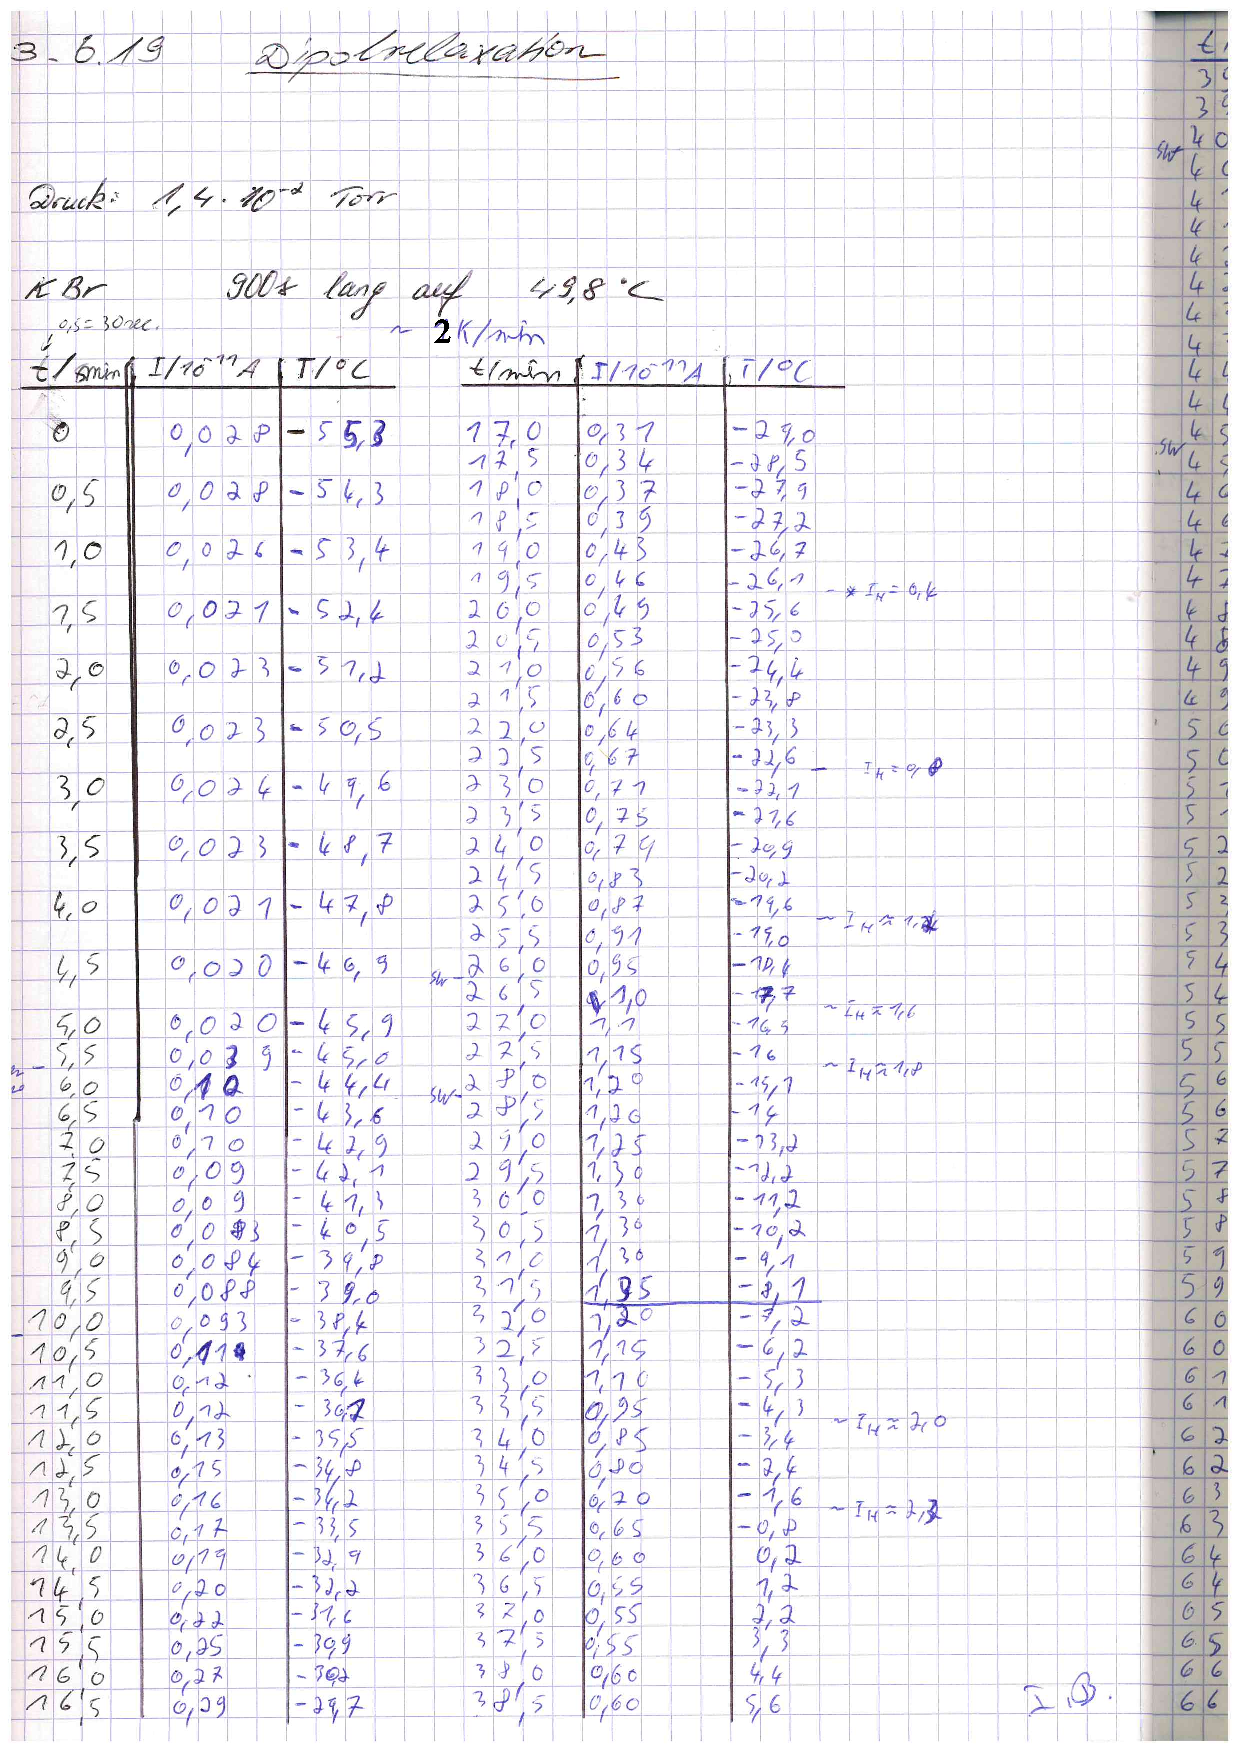
\includegraphics[width=\textwidth]{Messdaten1.pdf}
  \caption{Die Messdaten für eine Heizrate von etwa \SI{1}{\kelvin\per\minute}. Nicht verwendete Messdaten sind blau und die für den Untergrundverwendeten grün dargestellt. Die lila Linien makieren den betrachtete Bereich.}
  \label{fig:Messdaten1}
\end{figure}
\begin{figure}[htb]
  \centering
  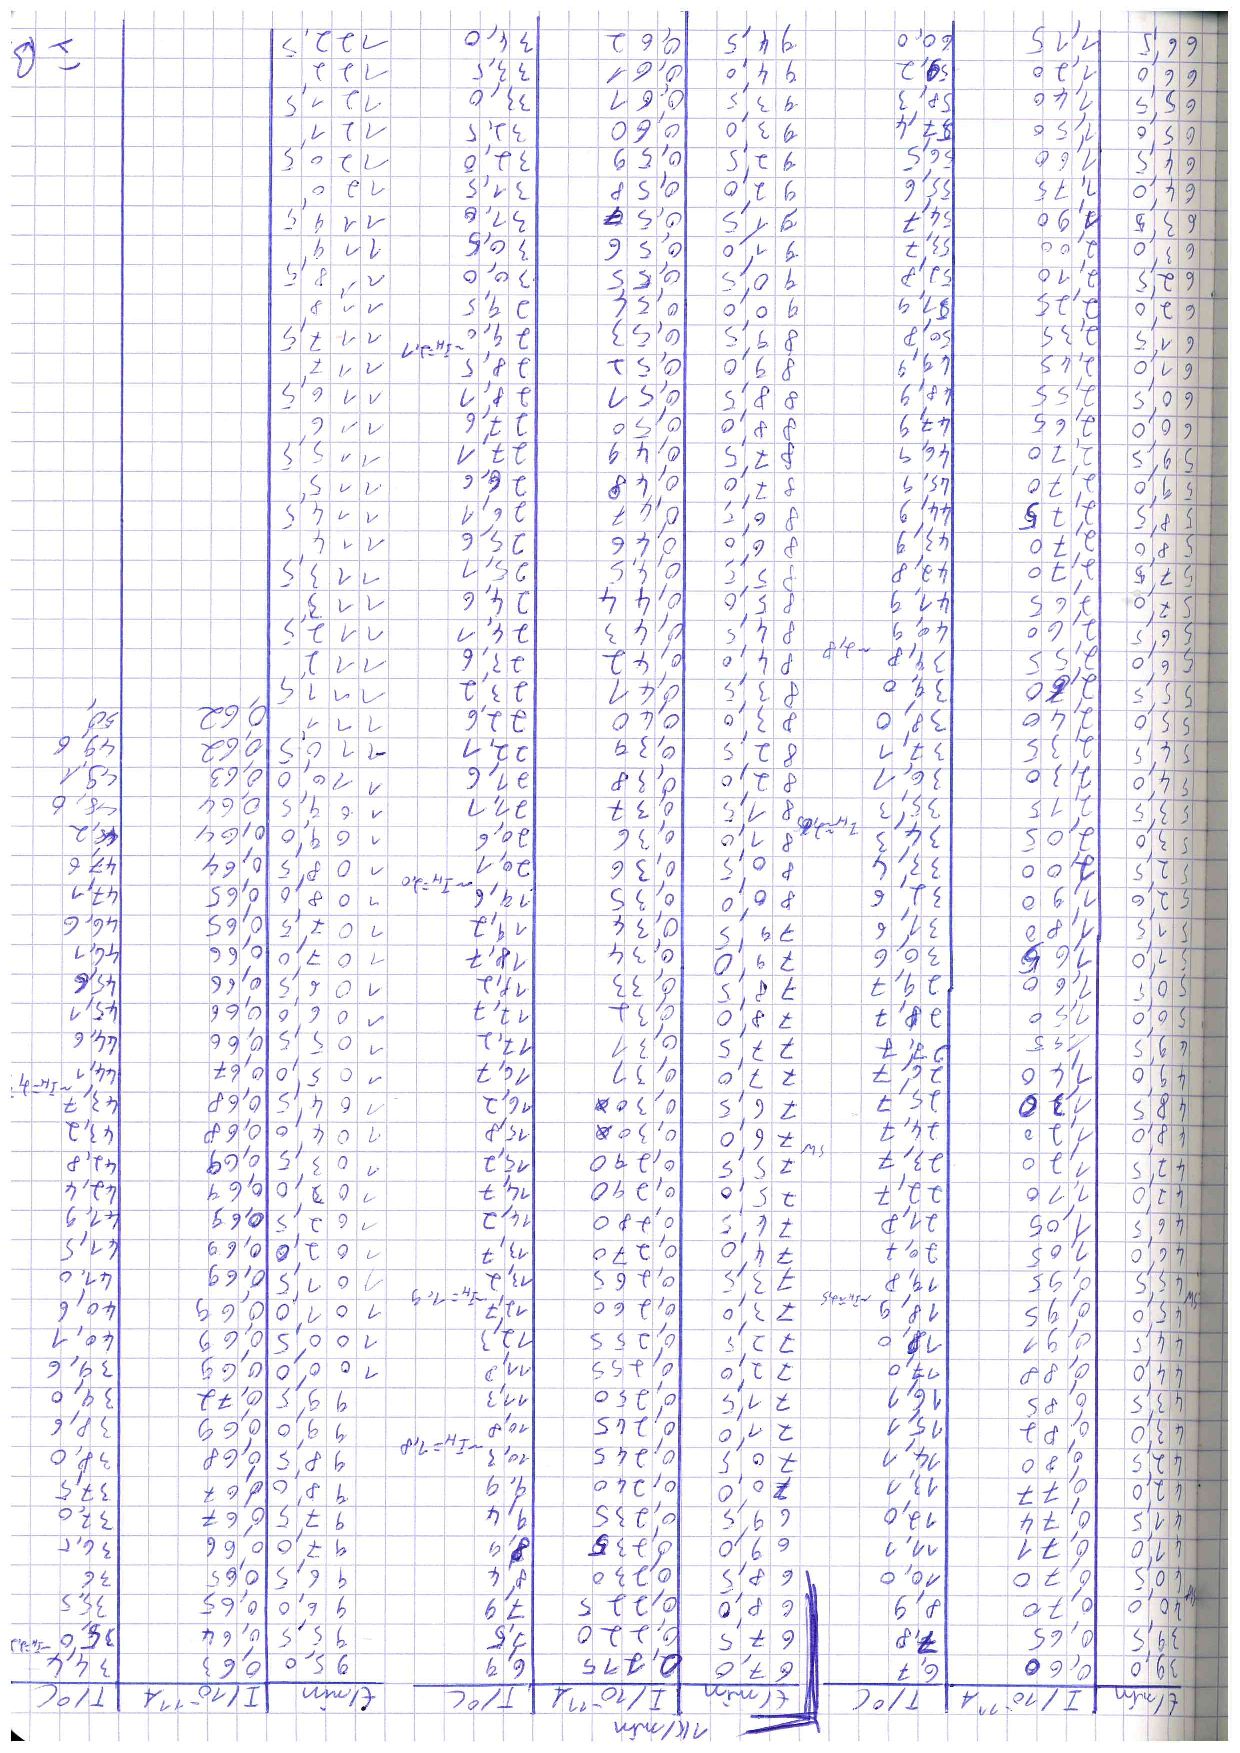
\includegraphics[width=\textwidth]{Messdaten2.pdf}
  \caption{Die Messdaten für eine Heizrate von etwa \SI{2}{\kelvin\per\minute}. Nicht verwendete Messdaten sind blau und die für den Untergrundverwendeten grün dargestellt. Die lila Linien makieren den betrachtete Bereich.}
  \label{fig:Messdaten2}
\end{figure}
\FloatBarrier

\subsection{Kleine Temperaturen}
\label{sec:klT}
Zur Berechnung der Aktivierungsenergie $W$ 

% \subsection{Unterkapiel}
% \label{sec:Unterkapitel}

% \begin{figure}[htb]
%   \centering
%   \includegraphics[width=\textwidth]{Plot.pdf}
%   \caption{Bildunterschrift}
%   \label{fig:Plot1}
% \end{figure}
\FloatBarrier